% Options for packages loaded elsewhere
\PassOptionsToPackage{unicode}{hyperref}
\PassOptionsToPackage{hyphens}{url}
%
\documentclass[
]{article}
\title{Uncertainty in times of COVID-19: Raw survey data}
\author{Fabian Lange, Lars Vilhuber}
\date{2022-06-03}

\usepackage{amsmath,amssymb}
\usepackage{lmodern}
\usepackage{iftex}
\ifPDFTeX
  \usepackage[T1]{fontenc}
  \usepackage[utf8]{inputenc}
  \usepackage{textcomp} % provide euro and other symbols
\else % if luatex or xetex
  \usepackage{unicode-math}
  \defaultfontfeatures{Scale=MatchLowercase}
  \defaultfontfeatures[\rmfamily]{Ligatures=TeX,Scale=1}
\fi
% Use upquote if available, for straight quotes in verbatim environments
\IfFileExists{upquote.sty}{\usepackage{upquote}}{}
\IfFileExists{microtype.sty}{% use microtype if available
  \usepackage[]{microtype}
  \UseMicrotypeSet[protrusion]{basicmath} % disable protrusion for tt fonts
}{}
\makeatletter
\@ifundefined{KOMAClassName}{% if non-KOMA class
  \IfFileExists{parskip.sty}{%
    \usepackage{parskip}
  }{% else
    \setlength{\parindent}{0pt}
    \setlength{\parskip}{6pt plus 2pt minus 1pt}}
}{% if KOMA class
  \KOMAoptions{parskip=half}}
\makeatother
\usepackage{xcolor}
\IfFileExists{xurl.sty}{\usepackage{xurl}}{} % add URL line breaks if available
\IfFileExists{bookmark.sty}{\usepackage{bookmark}}{\usepackage{hyperref}}
\hypersetup{
  pdftitle={Uncertainty in times of COVID-19: Raw survey data},
  pdfauthor={Fabian Lange, Lars Vilhuber},
  hidelinks,
  pdfcreator={LaTeX via pandoc}}
\urlstyle{same} % disable monospaced font for URLs
\usepackage[margin=1in]{geometry}
\usepackage{longtable,booktabs,array}
\usepackage{calc} % for calculating minipage widths
% Correct order of tables after \paragraph or \subparagraph
\usepackage{etoolbox}
\makeatletter
\patchcmd\longtable{\par}{\if@noskipsec\mbox{}\fi\par}{}{}
\makeatother
% Allow footnotes in longtable head/foot
\IfFileExists{footnotehyper.sty}{\usepackage{footnotehyper}}{\usepackage{footnote}}
\makesavenoteenv{longtable}
\usepackage{graphicx}
\makeatletter
\def\maxwidth{\ifdim\Gin@nat@width>\linewidth\linewidth\else\Gin@nat@width\fi}
\def\maxheight{\ifdim\Gin@nat@height>\textheight\textheight\else\Gin@nat@height\fi}
\makeatother
% Scale images if necessary, so that they will not overflow the page
% margins by default, and it is still possible to overwrite the defaults
% using explicit options in \includegraphics[width, height, ...]{}
\setkeys{Gin}{width=\maxwidth,height=\maxheight,keepaspectratio}
% Set default figure placement to htbp
\makeatletter
\def\fps@figure{htbp}
\makeatother
\setlength{\emergencystretch}{3em} % prevent overfull lines
\providecommand{\tightlist}{%
  \setlength{\itemsep}{0pt}\setlength{\parskip}{0pt}}
\setcounter{secnumdepth}{-\maxdimen} % remove section numbering
\usepackage{titling}
\pretitle{\begin{center}\LARGE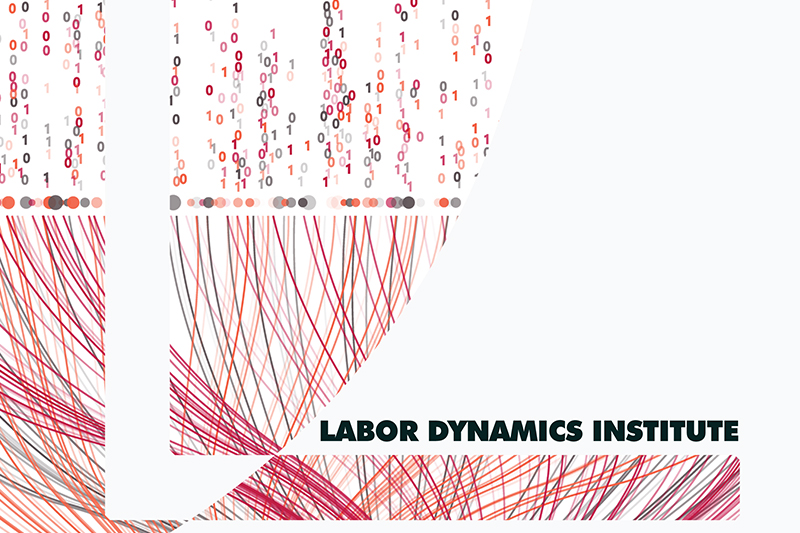
\includegraphics[width=10cm]{_includes/LDIimage.png}\\[\bigskipamount]}
\posttitle{\end{center}}
\ifLuaTeX
  \usepackage{selnolig}  % disable illegal ligatures
\fi

\begin{document}
\maketitle

{
\setcounter{tocdepth}{2}
\tableofcontents
}
\href{https://doi.org/10.5281/zenodo.3966534}{\includegraphics{https://zenodo.org/badge/DOI/10.5281/zenodo.3966534.svg}}

Data from a survey of consumer expectations

\hypertarget{description}{%
\subsection{Description}\label{description}}

From April 24, 2020, through June 22, 2020,
\href{http://www.fabianlange.ca/}{Fabian Lange} and
\href{https://lars.vilhuber.com}{Lars Vilhuber} conducted the survey
``Uncertainty in COVID-19 times.'' The survey is a single-question
survey focusing on people's anticipation about social distancing rules
and firm closures during the 2020 COVID-19 health crisis.

We believe that this information is not otherwise available in a
reliable and timely fashion. The information should be usable by
policy-makers and researchers, to be included in models of future
developments of society and the economy.

\hypertarget{citation}{%
\subsubsection{Citation}\label{citation}}

Please cite the data as

\begin{quote}
Lange, Fabian and Lars Vilhuber. 2020. ``Uncertainty in times of
COVID-19: Raw survey data {[}dataset{]}.'' Available at
\url{https://doi.org/10.5281/zenodo.3966534}.
\end{quote}

Please cite this document as

\begin{quote}
Lange, Fabian and Lars Vilhuber. 2020. ``Codebook for: Uncertainty in
times of COVID-19: Raw survey data.'' Available at
\url{https://doi.org/10.5281/zenodo.3966534} and
\url{https://labordynamicsinstitute.github.io//covid19-expectations-data}
(accessed 2022-06-03).
\end{quote}

Data is archived as of the last survey week on Zenodo:
\url{https://doi.org/10.5281/zenodo.3966534}.

\hypertarget{available-data}{%
\subsection{Available data}\label{available-data}}

\hypertarget{final-files}{%
\subsubsection{Final files}\label{final-files}}

Final files are uploaded after each wave is completed. Filenames in
\href{final/}{\texttt{final}} tagged with geography, language, the
question type,and date downloaded:

\begin{quote}
\texttt{survey-{[}geography{]}-{[}language{]}-{[}question{]}-{[}date{]}.xlsx}
\end{quote}

\hypertarget{list-of-files}{%
\subsubsection{List of files}\label{list-of-files}}

\begin{longtable}[]{@{}l@{}}
\toprule
Files \\
\midrule
\endhead
\href{final/survey-canada-en-businesses-20200506.xlsx}{survey-canada-en-businesses-20200506.xlsx} \\
\href{final/survey-canada-en-businesses-20200508.xlsx}{survey-canada-en-businesses-20200508.xlsx} \\
\href{final/survey-canada-en-businesses-20200515.xlsx}{survey-canada-en-businesses-20200515.xlsx} \\
\href{final/survey-canada-en-businesses-20200522.xlsx}{survey-canada-en-businesses-20200522.xlsx} \\
\href{final/survey-canada-en-businesses-20200529.xlsx}{survey-canada-en-businesses-20200529.xlsx} \\
\href{final/survey-canada-en-businesses-20200605.xlsx}{survey-canada-en-businesses-20200605.xlsx} \\
\href{final/survey-canada-en-businesses-20200612.xlsx}{survey-canada-en-businesses-20200612.xlsx} \\
\href{final/survey-canada-en-businesses-20200619.xlsx}{survey-canada-en-businesses-20200619.xlsx} \\
\href{final/survey-canada-en-people-20200503.xlsx}{survey-canada-en-people-20200503.xlsx} \\
\href{final/survey-canada-en-people-20200508.xlsx}{survey-canada-en-people-20200508.xlsx} \\
\href{final/survey-canada-en-people-20200515.xlsx}{survey-canada-en-people-20200515.xlsx} \\
\href{final/survey-canada-en-people-20200522.xlsx}{survey-canada-en-people-20200522.xlsx} \\
\href{final/survey-canada-en-people-20200529.xlsx}{survey-canada-en-people-20200529.xlsx} \\
\href{final/survey-canada-en-people-20200605.xlsx}{survey-canada-en-people-20200605.xlsx} \\
\href{final/survey-canada-en-people-20200612.xlsx}{survey-canada-en-people-20200612.xlsx} \\
\href{final/survey-canada-fr-businesses-20200426.xlsx}{survey-canada-fr-businesses-20200426.xlsx} \\
\href{final/survey-canada-fr-people-20200426.xlsx}{survey-canada-fr-people-20200426.xlsx} \\
\href{final/survey-ny-en-businesses-20200512.xlsx}{survey-ny-en-businesses-20200512.xlsx} \\
\href{final/survey-ny-en-businesses-20200527.xlsx}{survey-ny-en-businesses-20200527.xlsx} \\
\href{final/survey-ny-en-people-20200513.xlsx}{survey-ny-en-people-20200513.xlsx} \\
\href{final/survey-ny-en-people-20200527.xlsx}{survey-ny-en-people-20200527.xlsx} \\
\href{final/survey-qc-fr-businesses-20200429.xlsx}{survey-qc-fr-businesses-20200429.xlsx} \\
\href{final/survey-qc-fr-businesses-20200503.xlsx}{survey-qc-fr-businesses-20200503.xlsx} \\
\href{final/survey-qc-fr-businesses-20200510.xlsx}{survey-qc-fr-businesses-20200510.xlsx} \\
\href{final/survey-qc-fr-businesses-20200517.xlsx}{survey-qc-fr-businesses-20200517.xlsx} \\
\href{final/survey-qc-fr-businesses-20200524.xlsx}{survey-qc-fr-businesses-20200524.xlsx} \\
\href{final/survey-qc-fr-businesses-20200530.xlsx}{survey-qc-fr-businesses-20200530.xlsx} \\
\href{final/survey-qc-fr-businesses-20200607.xlsx}{survey-qc-fr-businesses-20200607.xlsx} \\
\href{final/survey-qc-fr-businesses-20200614.xlsx}{survey-qc-fr-businesses-20200614.xlsx} \\
\href{final/survey-qc-fr-people-20200429.xlsx}{survey-qc-fr-people-20200429.xlsx} \\
\href{final/survey-qc-fr-people-20200503.xlsx}{survey-qc-fr-people-20200503.xlsx} \\
\href{final/survey-qc-fr-people-20200510.xlsx}{survey-qc-fr-people-20200510.xlsx} \\
\href{final/survey-qc-fr-people-20200517.xlsx}{survey-qc-fr-people-20200517.xlsx} \\
\href{final/survey-qc-fr-people-20200524.xlsx}{survey-qc-fr-people-20200524.xlsx} \\
\href{final/survey-qc-fr-people-20200529.xlsx}{survey-qc-fr-people-20200529.xlsx} \\
\href{final/survey-qc-fr-people-20200607.xlsx}{survey-qc-fr-people-20200607.xlsx} \\
\href{final/survey-qc-fr-people-20200614.xlsx}{survey-qc-fr-people-20200614.xlsx} \\
\href{final/survey-us-en-businesses-20200429.xlsx}{survey-us-en-businesses-20200429.xlsx} \\
\href{final/survey-us-en-businesses-20200503.xlsx}{survey-us-en-businesses-20200503.xlsx} \\
\href{final/survey-us-en-businesses-20200511.xlsx}{survey-us-en-businesses-20200511.xlsx} \\
\href{final/survey-us-en-businesses-20200517.xlsx}{survey-us-en-businesses-20200517.xlsx} \\
\href{final/survey-us-en-businesses-20200524.xlsx}{survey-us-en-businesses-20200524.xlsx} \\
\href{final/survey-us-en-businesses-20200601.xlsx}{survey-us-en-businesses-20200601.xlsx} \\
\href{final/survey-us-en-businesses-20200607.xlsx}{survey-us-en-businesses-20200607.xlsx} \\
\href{final/survey-us-en-businesses-20200614.xlsx}{survey-us-en-businesses-20200614.xlsx} \\
\href{final/survey-us-en-people-20200429.xlsx}{survey-us-en-people-20200429.xlsx} \\
\href{final/survey-us-en-people-20200504.xlsx}{survey-us-en-people-20200504.xlsx} \\
\href{final/survey-us-en-people-20200510.xlsx}{survey-us-en-people-20200510.xlsx} \\
\href{final/survey-us-en-people-20200517.xlsx}{survey-us-en-people-20200517.xlsx} \\
\href{final/survey-us-en-people-20200525.xlsx}{survey-us-en-people-20200525.xlsx} \\
\href{final/survey-us-en-people-20200601.xlsx}{survey-us-en-people-20200601.xlsx} \\
\href{final/survey-us-en-people-20200609.xlsx}{survey-us-en-people-20200609.xlsx} \\
\bottomrule
\end{longtable}

\hypertarget{normalized-files}{%
\subsubsection{Normalized files}\label{normalized-files}}

We provide a normalized Stata and R (\texttt{Rds}) file with all
surveys, recoded consistently.

\begin{longtable}[]{@{}l@{}}
\toprule
Files \\
\midrule
\endhead
\href{derived/expectations.csv}{expectations.csv} \\
\href{derived/expectations.dta}{expectations.dta} \\
\href{derived/expectations.Rds}{expectations.Rds} \\
\bottomrule
\end{longtable}

\hypertarget{auxiliary-files}{%
\subsubsection{Auxiliary files}\label{auxiliary-files}}

We provide additional files that were either used or generated in the
process of data cleaning, in particular for the reweighting.
(explanations to come)

\begin{longtable}[]{@{}l@{}}
\toprule
Files \\
\midrule
\endhead
\href{auxiliary/aggregage_agegrp_ca.xlsx}{aggregage\_agegrp\_ca.xlsx} \\
\href{auxiliary/reweights_aux_ca.csv}{reweights\_aux\_ca.csv} \\
\href{auxiliary/reweights_aux_ca.dta}{reweights\_aux\_ca.dta} \\
\href{auxiliary/reweights_aux_ca.Rds}{reweights\_aux\_ca.Rds} \\
\href{auxiliary/reweights_aux_us.csv}{reweights\_aux\_us.csv} \\
\href{auxiliary/reweights_aux_us.dta}{reweights\_aux\_us.dta} \\
\href{auxiliary/reweights_aux_us.Rds}{reweights\_aux\_us.Rds} \\
\href{auxiliary/standardize_values.xlsx}{standardize\_values.xlsx} \\
\href{auxiliary/statcan_regions_2011_table8.xlsx}{statcan\_regions\_2011\_table8.xlsx} \\
\href{auxiliary/state-geocodes-v2017.xlsx}{state-geocodes-v2017.xlsx} \\
\bottomrule
\end{longtable}

\hypertarget{temporary-files}{%
\subsubsection{Temporary files}\label{temporary-files}}

Temporary files may be made available if a survey has not yet completed,
but data are already available.

\href{temporary/}{\texttt{Temporary}} files follow

\begin{quote}
\texttt{survey-{[}surveyid{]}.xlsx}
\end{quote}

\hypertarget{data-description}{%
\subsection{Data description}\label{data-description}}

\begin{longtable}[]{@{}
  >{\raggedright\arraybackslash}p{(\columnwidth - 2\tabcolsep) * \real{0.50}}
  >{\raggedright\arraybackslash}p{(\columnwidth - 2\tabcolsep) * \real{0.50}}@{}}
\toprule
\begin{minipage}[b]{\linewidth}\raggedright
Topic
\end{minipage} & \begin{minipage}[b]{\linewidth}\raggedright
Answer
\end{minipage} \\
\midrule
\endhead
Geographic Coverage & United States of America, Canada \\
Time Periods & 2020-04-24 - 2020-06-19 \\
Date of Collection & 2020-04-24 - 2020-06-19 \\
Unit of Observation & Individual \\
Description of Variables & User\_ID, Time\_UTC, Survey\_Completion,
Publisher\_Category, Gender, Age, Geography, Weight,
Question\_1\_Answer, rt\_Q1\_ms \\
\bottomrule
\end{longtable}

\hypertarget{reference-period}{%
\subsubsection{Reference period}\label{reference-period}}

The survey asks about point-in-time expectations. A new wave is launched
every Friday. The list provides the dates of collection for each wave.
Currently, data are available covering the period between 2020-04-24 and
2020-06-19.

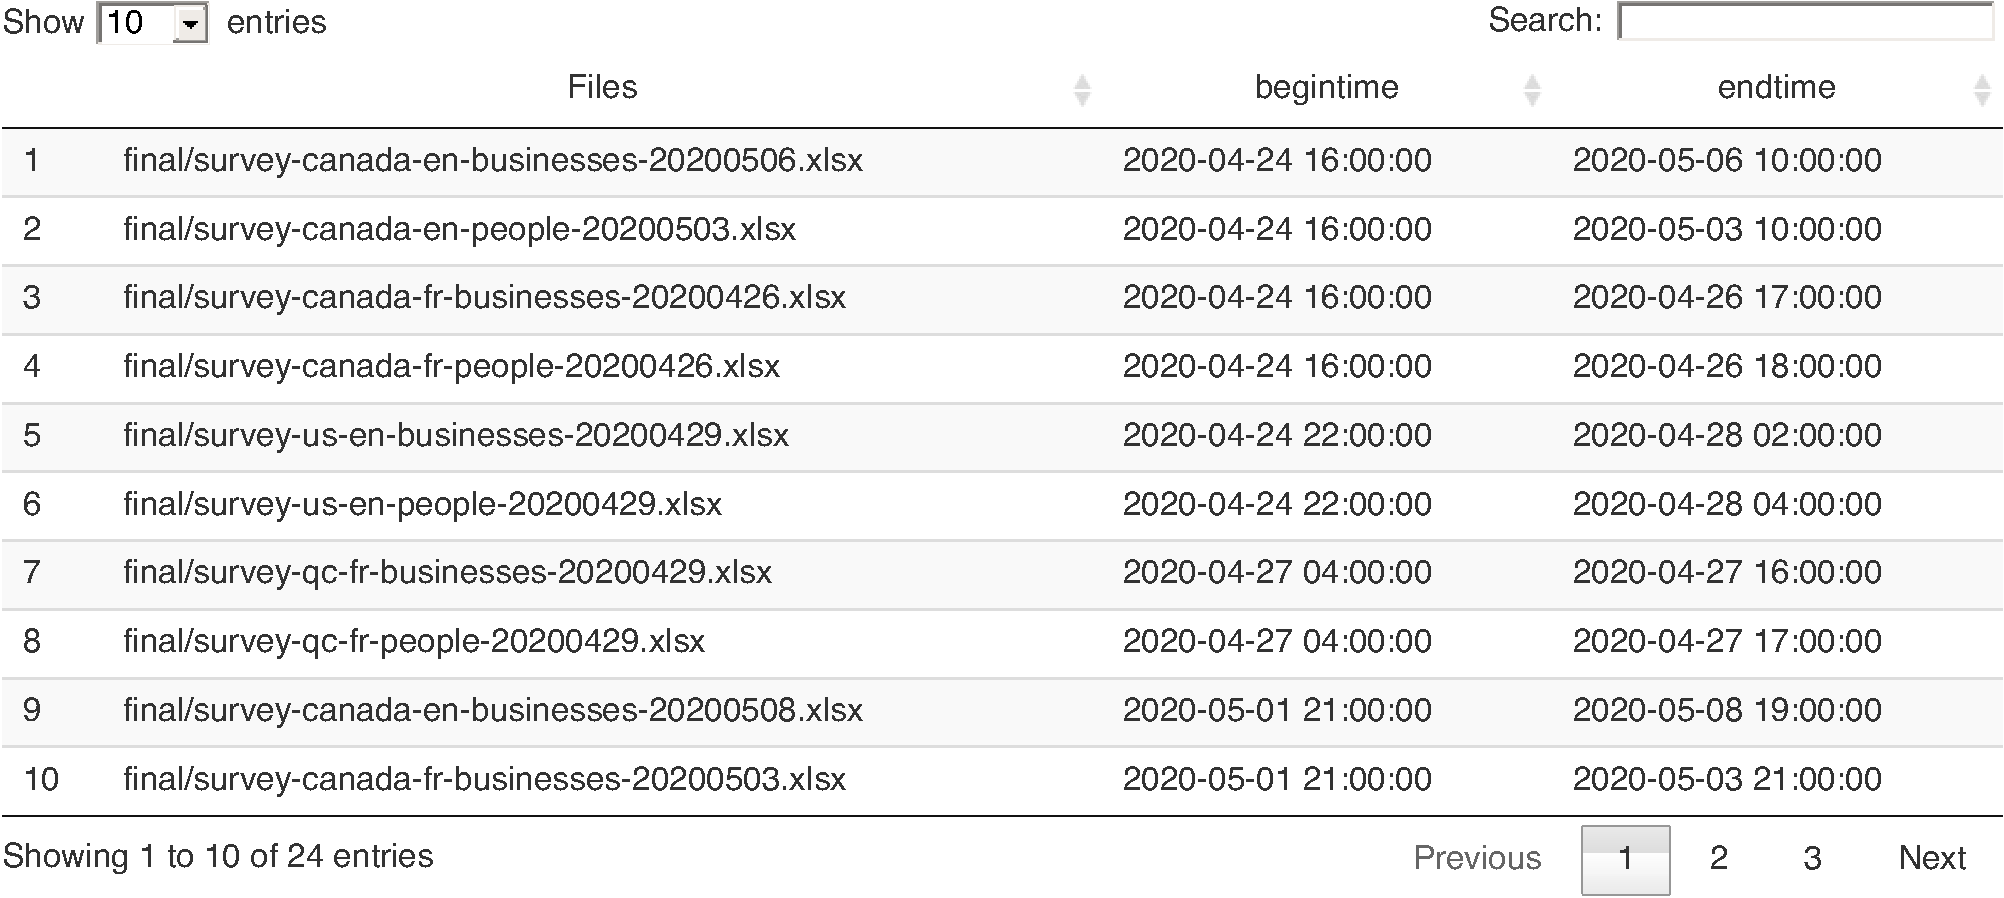
\includegraphics{expectations-codebook_files/figure-latex/unnamed-chunk-2-1.pdf}

\hypertarget{data-dictionary}{%
\subsubsection{Data Dictionary}\label{data-dictionary}}

\hypertarget{q1-answer-to-primary-question}{%
\paragraph{Q1: Answer to primary
question}\label{q1-answer-to-primary-question}}

This field captures the answer to the
\protect\hyperlink{question-type}{sole question of each survey}, where
answers differ across geographic scope (\texttt{geotag}), and languages.
A consolidated (standardized) distribution is shown below, using the
\href{auxiliary/standardize_values.xlsx}{standardizer mapping}.

\hypertarget{standardized-distribution}{%
\subparagraph{Standardized
distribution}\label{standardized-distribution}}

The following tabulations are of unweighted data.

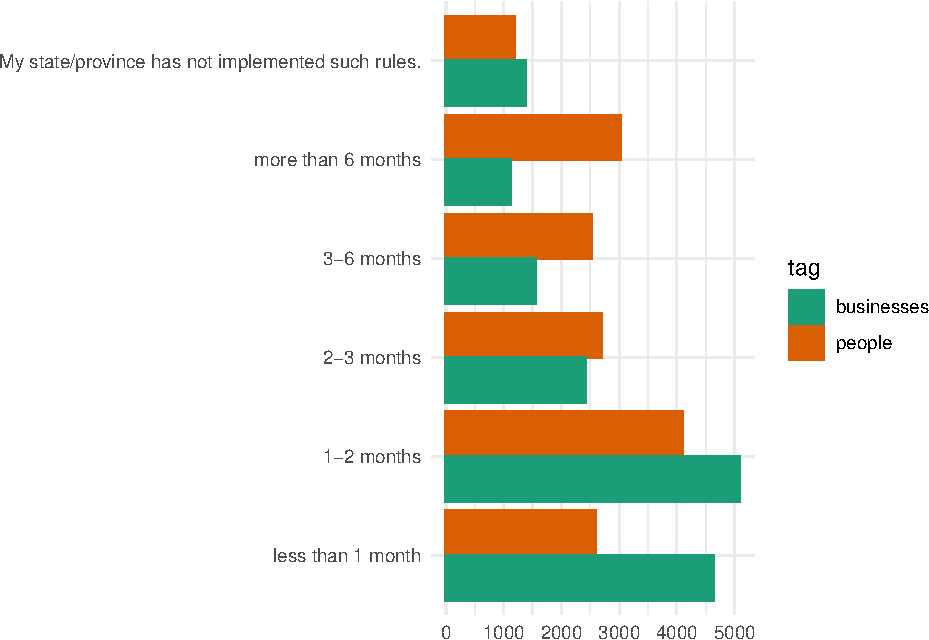
\includegraphics{expectations-codebook_files/figure-latex/graph-1.pdf}

\hypertarget{people-canada-english}{%
\subparagraph{People, Canada, English}\label{people-canada-english}}

\begin{longtable}[]{@{}lrr@{}}
\toprule
Question\_1\_Answer & count & percent \\
\midrule
\endhead
1-2 months & 2561 & 21.23 \\
2-3 months & 2015 & 16.71 \\
3-6 months & 1986 & 16.46 \\
less than 1 month & 1559 & 12.92 \\
more than 6 months & 2674 & 22.17 \\
My province has not implemented such rules. & 1267 & 10.50 \\
\bottomrule
\end{longtable}

\hypertarget{business-canada-french}{%
\subparagraph{Business, Canada, French}\label{business-canada-french}}

\begin{longtable}[]{@{}lrr@{}}
\toprule
Question\_1\_Answer & count & percent \\
\midrule
\endhead
1-2 mois & 1553 & 30.66 \\
2-3 mois & 1071 & 21.14 \\
3-6 mois & 769 & 15.18 \\
Les entreprises dans ma province ne sont pas fermées & 236 & 4.66 \\
moins d'un mois & 1130 & 22.31 \\
plus que 6 mois & 307 & 6.06 \\
\bottomrule
\end{longtable}

\hypertarget{people-canada-french}{%
\subparagraph{People, Canada, French}\label{people-canada-french}}

\begin{longtable}[]{@{}lrr@{}}
\toprule
Question\_1\_Answer & count & percent \\
\midrule
\endhead
1-2 mois & 842 & 17.02 \\
2-3 mois & 965 & 19.51 \\
3-6 mois & 1334 & 26.97 \\
Ma province n'a pas de telles mesures & 27 & 0.55 \\
moins d'un mois & 269 & 5.44 \\
plus que 6 mois & 1509 & 30.51 \\
\bottomrule
\end{longtable}

\hypertarget{business-us-english}{%
\subparagraph{Business, US, English}\label{business-us-english}}

\begin{longtable}[]{@{}lrr@{}}
\toprule
Question\_1\_Answer & count & percent \\
\midrule
\endhead
1-2 months & 5046 & 25.11 \\
2-3 months & 1918 & 9.55 \\
3-6 months & 1293 & 6.44 \\
less than 1 month & 8365 & 41.63 \\
more than 6 months & 1306 & 6.50 \\
My state has not implemented such rules. & 2165 & 10.77 \\
\bottomrule
\end{longtable}

\hypertarget{people-us-english}{%
\subparagraph{People, US, English}\label{people-us-english}}

\begin{longtable}[]{@{}lrr@{}}
\toprule
Question\_1\_Answer & count & percent \\
\midrule
\endhead
1-2 months & 4131 & 23.57 \\
2-3 months & 2411 & 13.76 \\
3-6 months & 2379 & 13.57 \\
less than 1 month & 3894 & 22.22 \\
more than 6 months & 3228 & 18.42 \\
My state has not implemented such rules. & 1485 & 8.47 \\
\bottomrule
\end{longtable}

\hypertarget{question-type}{%
\paragraph{Question type}\label{question-type}}

The actual question asked is encoded in the \texttt{tag} variable on
\protect\hyperlink{normalized-files}{normalized files}, and differs by
\protect\hyperlink{geographic-target}{geographic target}
(\texttt{geotag}). On the original files, geographic target is not
identifiable except through the file name, and the question text is on
the ``Overview'' tab. On the
\protect\hyperlink{normalized-files}{normalized files}, the variables
\texttt{tag} and \texttt{geotag} allow to map back to the actual
question:

\includegraphics{expectations-codebook_files/figure-latex/question_table-1.pdf}

\hypertarget{geographic-target}{%
\subparagraph{Geographic target}\label{geographic-target}}

Encoded in \texttt{geotag} on
\protect\hyperlink{normalized-files}{normalized files}, and specifies
the two-letter geocode (country or postal abbreviation) as targeted on
the Google Survey platform. Note: \texttt{geotag} = \texttt{qc} also
identifies the surveys that used the app.

\begin{longtable}[]{@{}lrr@{}}
\toprule
geotag & count & percent \\
\midrule
\endhead
canada & 26768 & 35.56 \\
ny & 2003 & 2.66 \\
qc & 8890 & 11.81 \\
us & 37621 & 49.97 \\
\bottomrule
\end{longtable}

\hypertarget{notes}{%
\subparagraph{Notes}\label{notes}}

\begin{itemize}
\tightlist
\item
  in Week 1 (2020-04-24), we ran a French-language app survey
  geo-targeted for Canada, and another one targeted at Québec only. In
  subsequent weeks, we ran the French-language app survey only in
  Québec.
\item
  in Week 3 (2020-05-10), we ran a supplementary web survey geo-targeted
  at New York State.
\end{itemize}

\hypertarget{age}{%
\paragraph{Age}\label{age}}

\begin{longtable}[]{@{}lrr@{}}
\toprule
Age & count & percent \\
\midrule
\endhead
18-24 & 9670 & 12.85 \\
25-34 & 12348 & 16.40 \\
35-44 & 10660 & 14.16 \\
45-54 & 9303 & 12.36 \\
55-64 & 9305 & 12.36 \\
65+ & 8902 & 11.82 \\
Unknown & 15094 & 20.05 \\
\bottomrule
\end{longtable}

\hypertarget{gender}{%
\paragraph{Gender}\label{gender}}

\begin{longtable}[]{@{}lrr@{}}
\toprule
Gender & count & percent \\
\midrule
\endhead
Female & 28419 & 37.75 \\
Male & 32794 & 43.56 \\
Unknown & 14069 & 18.69 \\
\bottomrule
\end{longtable}

\hypertarget{geography}{%
\paragraph{Geography}\label{geography}}

Geography is as coded by Google Surveys. Precision may vary, having
country, region, province, and sometimes city. Note that this may be
different from the \protect\hyperlink{geographic-target}{targeted
geography}.

\hypertarget{detailed-geography}{%
\subparagraph{Detailed geography}\label{detailed-geography}}

The variable \texttt{Geography} corresponds to the geography as captured
and recorded by Google. All other geography variables are derived from
this variable, and are only available on the
\protect\hyperlink{normalized-files}{normalized files}.

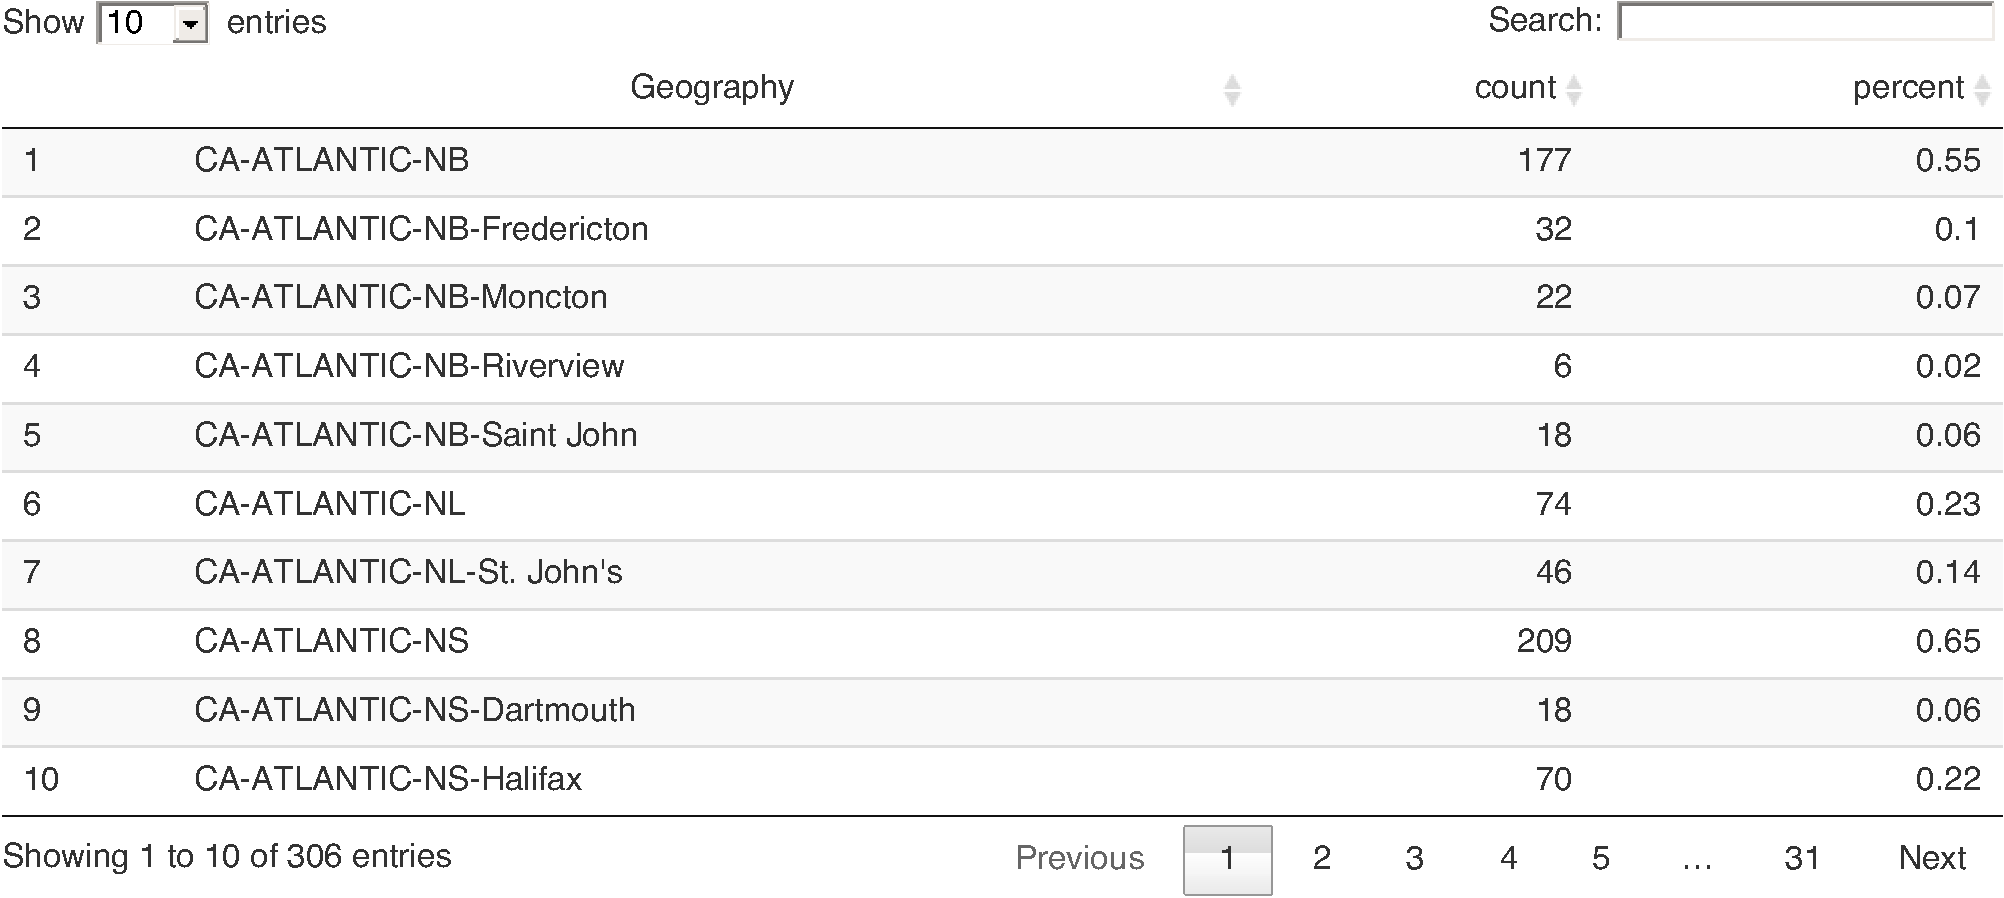
\includegraphics{expectations-codebook_files/figure-latex/details_geography-1.pdf}

\hypertarget{country}{%
\subparagraph{Country}\label{country}}

Distribution across countries

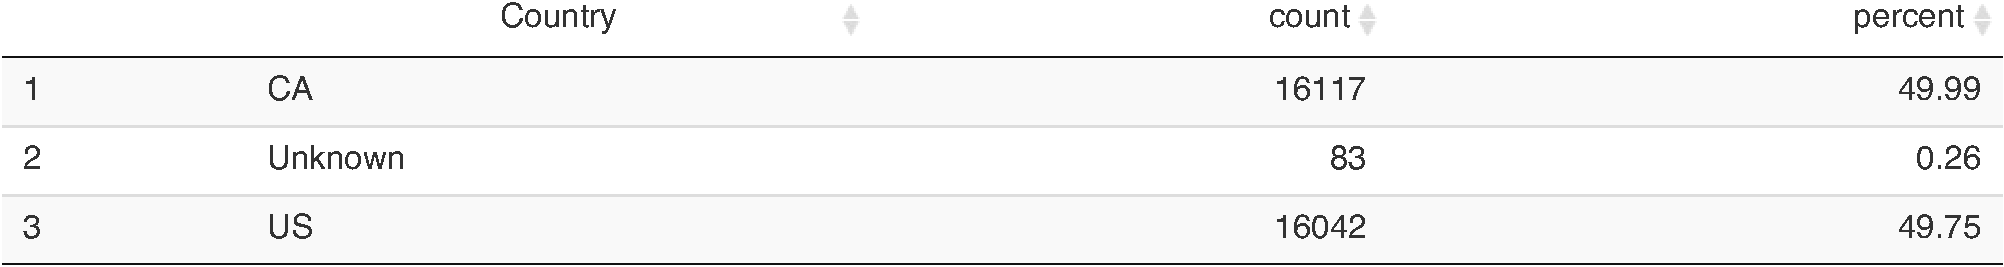
\includegraphics{expectations-codebook_files/figure-latex/details_country-1.pdf}

\hypertarget{region}{%
\subparagraph{Region}\label{region}}

Regions may be single states or provinces, or larger collections. They
may correspond to US Census regions or
\href{https://www12.statcan.gc.ca/census-recensement/2011/ref/dict/table-tableau/table-tableau-8-eng.cfm}{Statistics
Canada regions}.

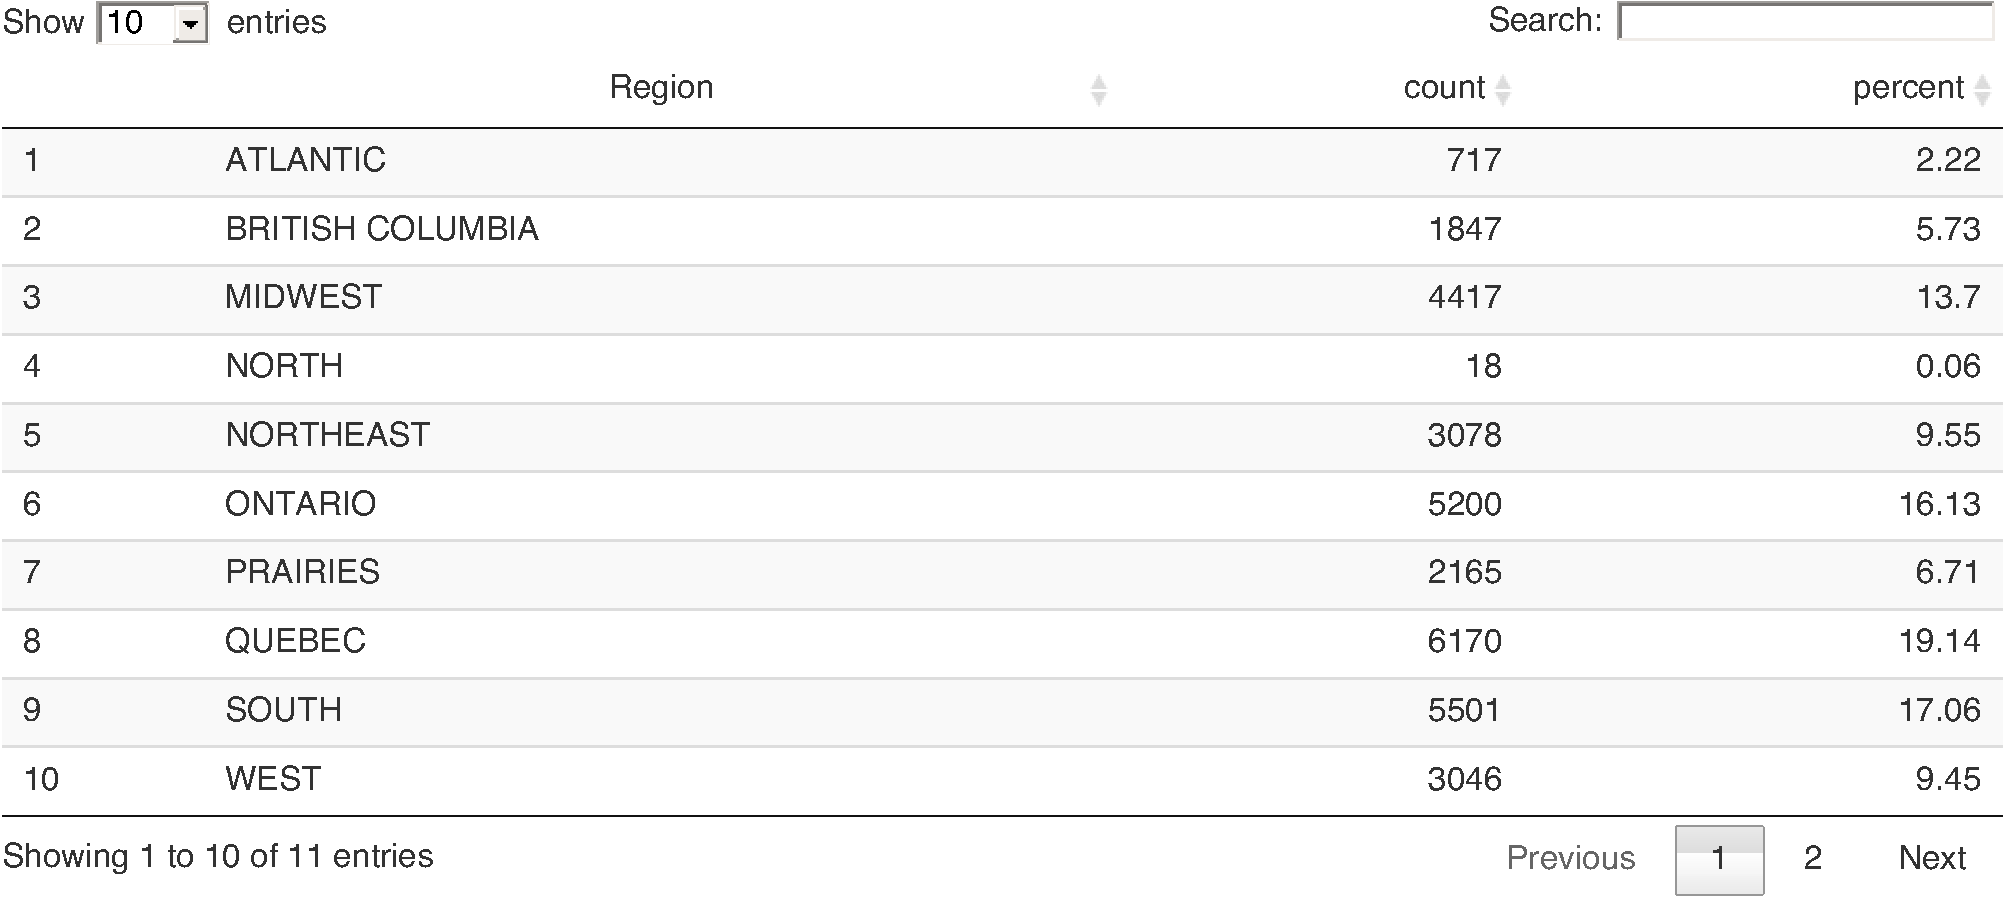
\includegraphics{expectations-codebook_files/figure-latex/details_regions-1.pdf}

\hypertarget{statesprovince}{%
\subparagraph{States/Province}\label{statesprovince}}

States and provinces are codes as two-letter postal abbreviation on the
original data files. On derived files, \texttt{geonum} contains the
numeric FIPS or
\href{https://www12.statcan.gc.ca/census-recensement/2011/ref/dict/table-tableau/table-tableau-8-eng.cfm}{province
code} (coded as character to preserve leading zeros), and as a full name
(\texttt{geoname}). Note that the Google-provided \texttt{Region} often,
but not always corresponds to a state or province, whereas
\texttt{State\_Province}, \texttt{geonum}, \texttt{geoname} always
correspond to state/province.

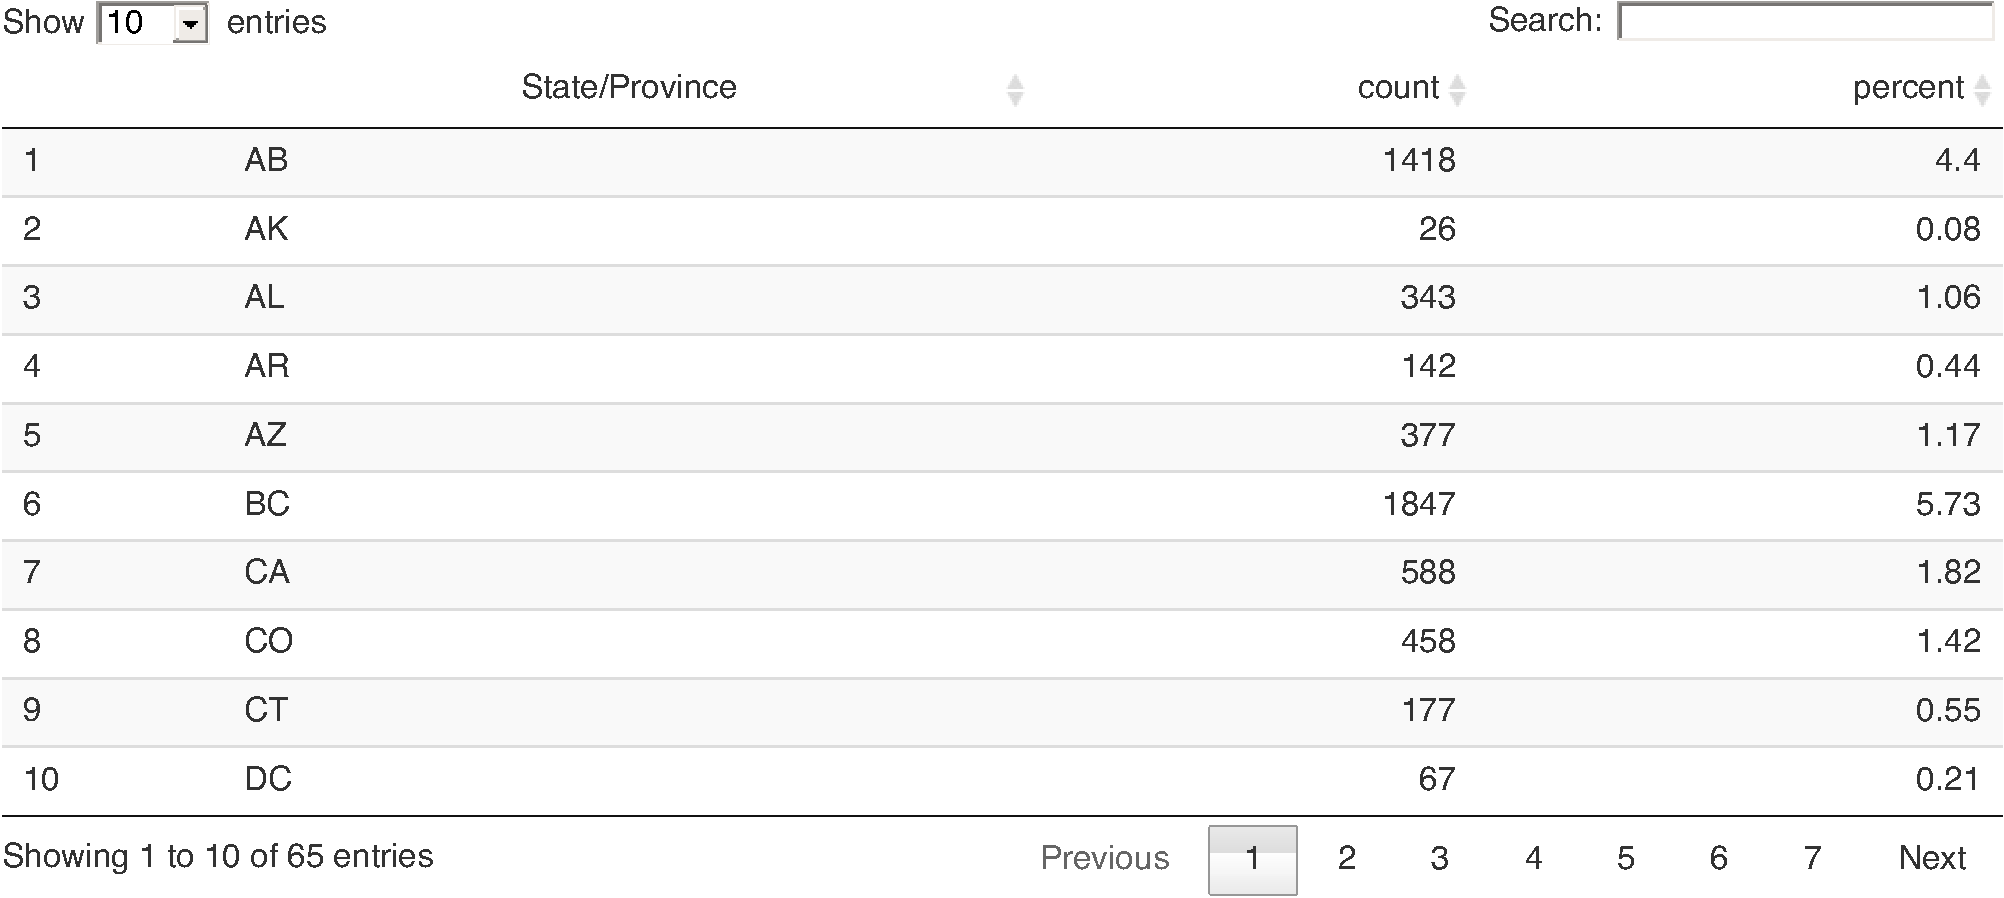
\includegraphics{expectations-codebook_files/figure-latex/details_state_province-1.pdf}

\hypertarget{city}{%
\subparagraph{City}\label{city}}

In some cases, details is available at the city level.

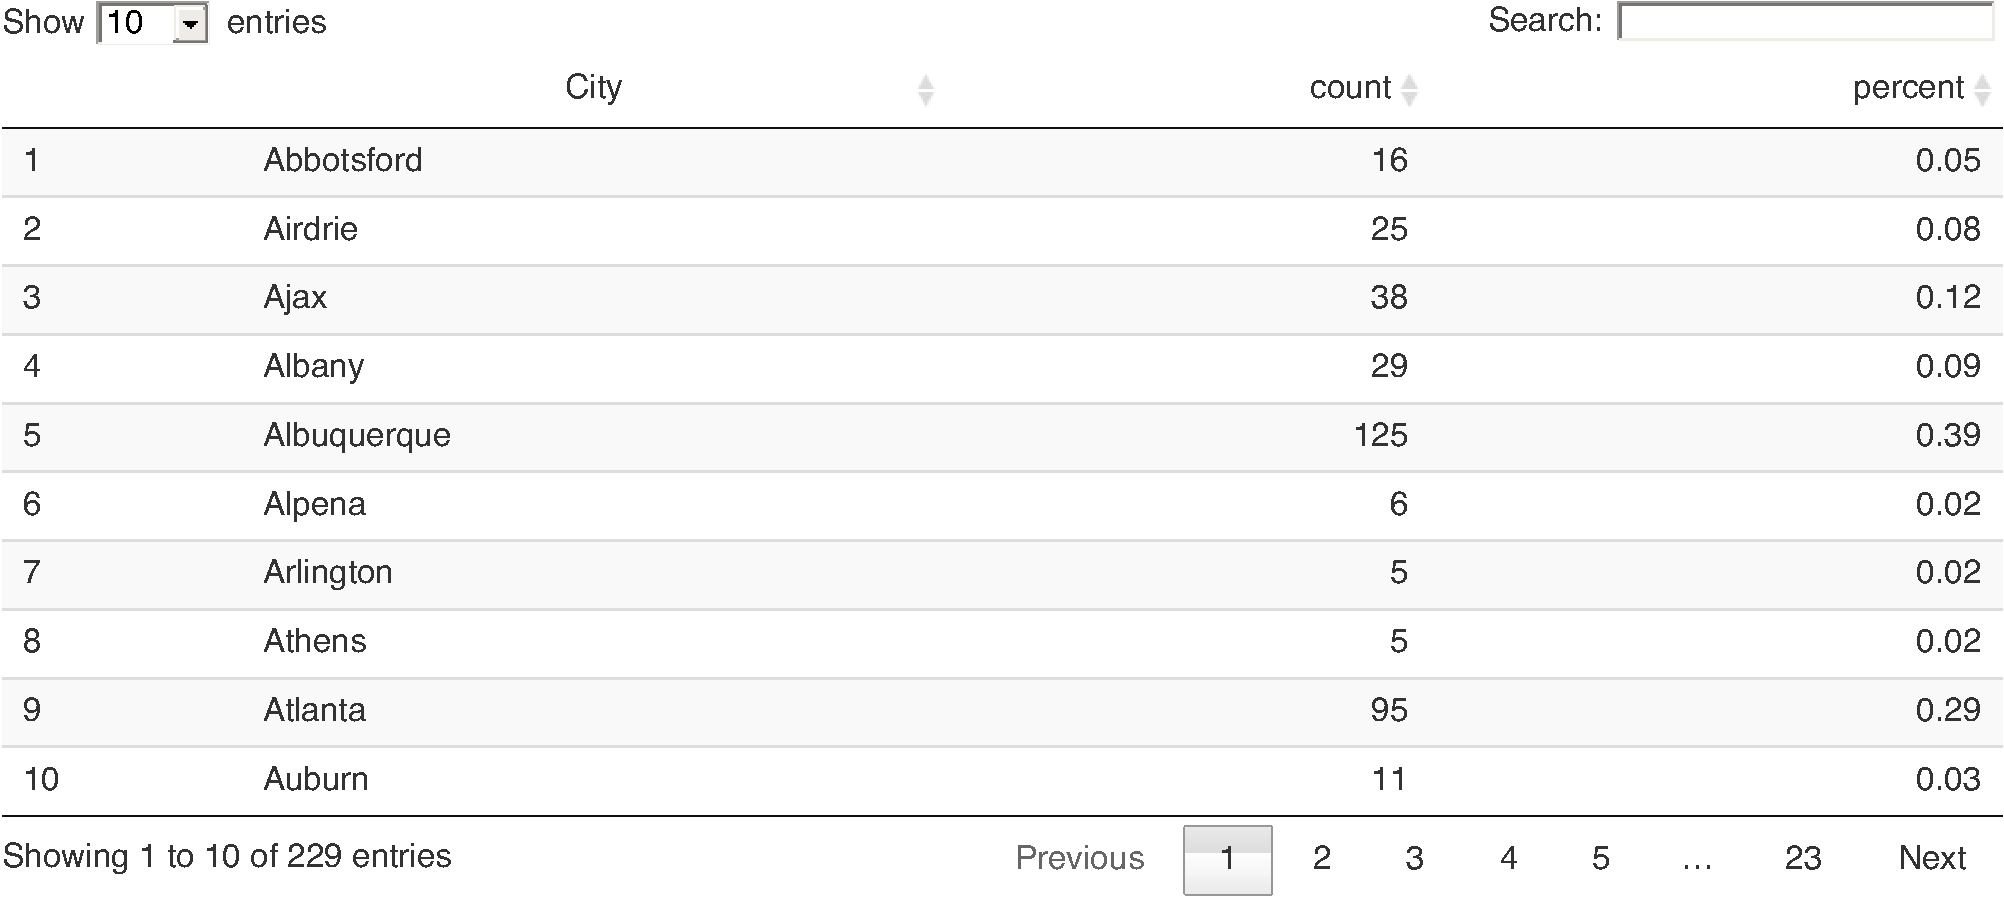
\includegraphics{expectations-codebook_files/figure-latex/details_cities-1.pdf}

\hypertarget{weight}{%
\paragraph{Weight}\label{weight}}

See \protect\hyperlink{weighting}{elsewhere in this document} how
weights are computed.

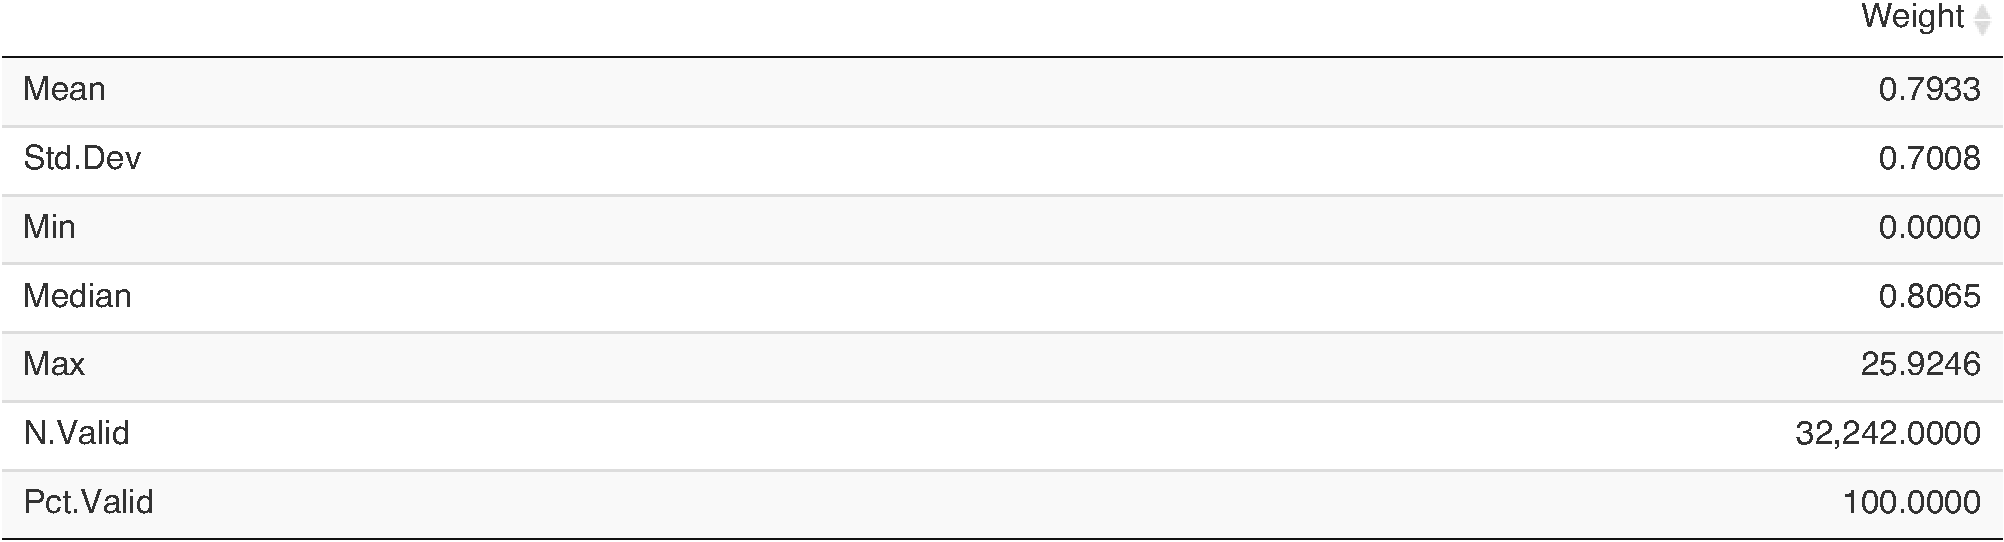
\includegraphics{expectations-codebook_files/figure-latex/details_weights-1.pdf}

\hypertarget{response-time}{%
\paragraph{Response Time}\label{response-time}}

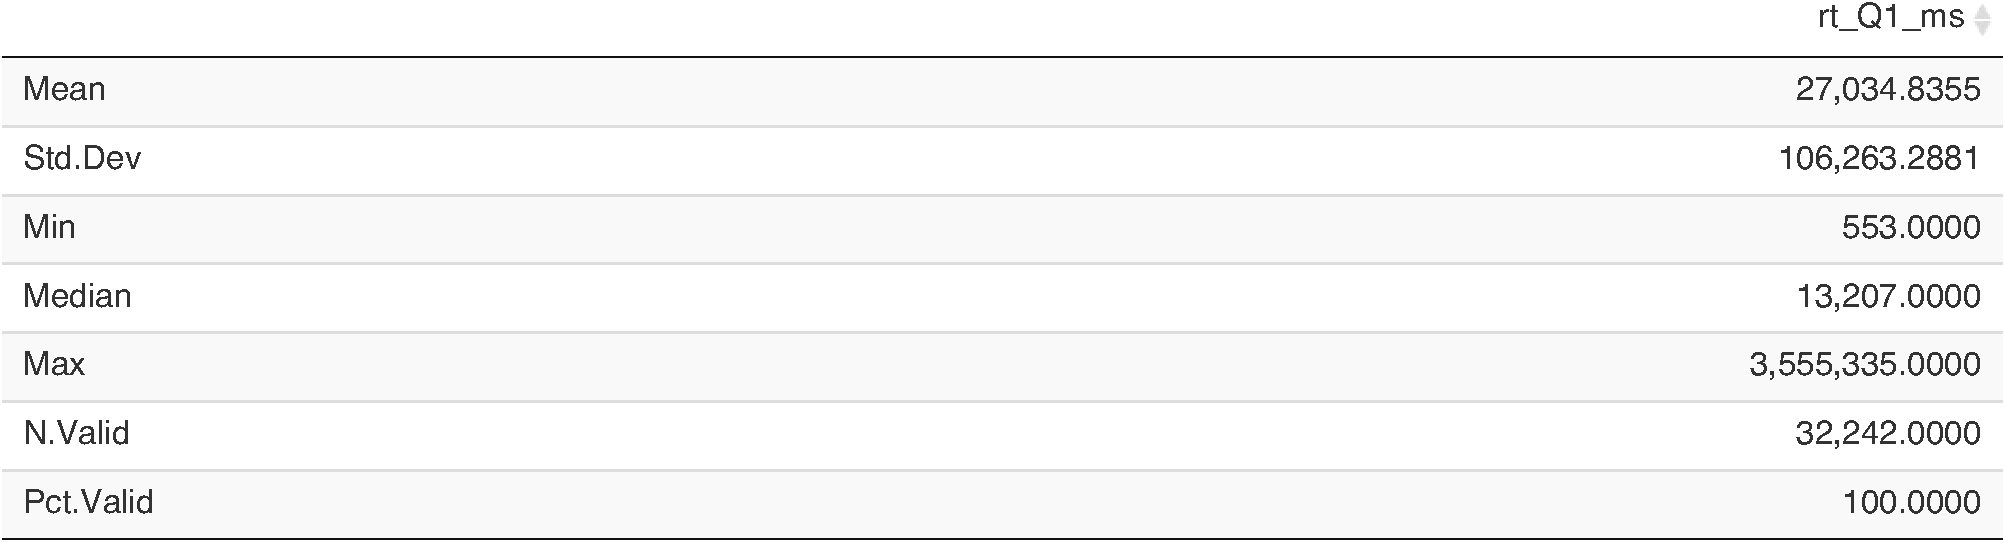
\includegraphics{expectations-codebook_files/figure-latex/details_responsetime-1.pdf}

\hypertarget{publisher-category}{%
\paragraph{Publisher Category}\label{publisher-category}}

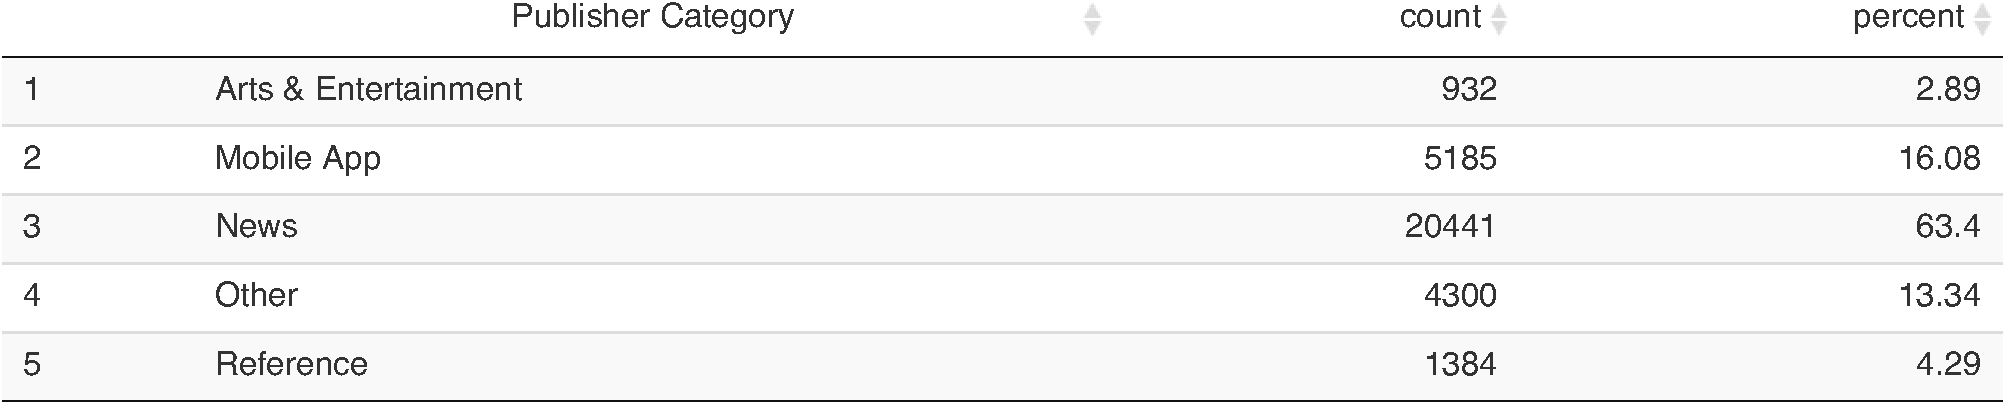
\includegraphics{expectations-codebook_files/figure-latex/details_publisher-1.pdf}

\hypertarget{not-tabulated}{%
\paragraph{Not tabulated}\label{not-tabulated}}

\begin{itemize}
\tightlist
\item
  \texttt{User\_ID}
\item
  \texttt{Time\_UTC}
\item
  \texttt{Survey\_Completion}
\end{itemize}

\hypertarget{data-structure}{%
\subsubsection{Data structure}\label{data-structure}}

Data files are available for each completed cycle of the survey, in
general once a week, and are stored under \href{final/}{\texttt{final}}.
Data from the preliminary study (assessing the questionnaire design) is
stored under \href{preliminary/}{\texttt{preliminary}}. We may make
available data before the survey is completed for each cycle, under
\href{temporary/}{\texttt{temporary}}, however, once the final version
from that cycle is available, these are deleted (this directory will be
empty on Zenodo).

\hypertarget{data-format}{%
\subsubsection{Data format}\label{data-format}}

Native format is Office Open XML (XLSX,
(\textbf{ecma\_international\_standard\_2016?}) ). Normalized files are
available in Stata and R formats.

Files are provided as downloaded from Google Surveys. Each file has 4
tabs.

\hypertarget{overview}{%
\paragraph{Overview}\label{overview}}

Lists the questions asked by the client, in this case Lange and
Vilhuber, as well as a survey ID.

\hypertarget{topline}{%
\paragraph{Topline}\label{topline}}

This tab contains a weighted summary of the responses to the questions
(similar to the above summary).

\hypertarget{complete-responses}{%
\paragraph{Complete responses}\label{complete-responses}}

This tab contains the actual microdata for any complete responses. Note
that for a single-question survey, this is identical to the ``All
responses.'' A complete response might have a weight of zero.

\hypertarget{all-responses}{%
\paragraph{All responses}\label{all-responses}}

All responses, whether complete or not, are recorded on this tab. In the
case of a single-question survey, this is identical to the ``Complete
responses'' tab.

\hypertarget{data-sources-and-methodology}{%
\subsection{Data sources and
methodology}\label{data-sources-and-methodology}}

\hypertarget{target-population}{%
\subsubsection{Target population}\label{target-population}}

\begin{itemize}
\tightlist
\item
  All Canadians aged 18 and older from the ten provinces and three
  territories are eligible to participate.
\item
  All US residents aged 18 and older are eligible to participate.
\end{itemize}

\hypertarget{instrument-design}{%
\subsubsection{Instrument design}\label{instrument-design}}

Each individual is asked one of two questions: how long they expect
``social distancing rules'' or ``business closures'' to remain in
effect:

\begin{itemize}
\tightlist
\item
  How much longer do you expect social distancing rules (restrictions on
  gatherings, stay-at-home rules) to stay in place in your
  province/state?
\item
  How much longer do you expect the closure of non-essential businesses
  to stay in place in your province/state?
\end{itemize}

Five response choices are offered:

\begin{itemize}
\tightlist
\item
  ``less than 1 month,''
\item
  ``1-2 months,''
\item
  ``2-3 months,''
\item
  ``3-6 months,''
\item
  ``more than 6 months.''
\end{itemize}

An additional answer allows respondents to affirm that ``such measures
are not implemented in their province/state.'' See
\protect\hyperlink{questionnaires}{questionnaires} for visual
representation of the questions.

\hypertarget{questionnaires}{%
\subsubsection{Questionnaires}\label{questionnaires}}

\hypertarget{data-collection}{%
\subsubsection{Data collection}\label{data-collection}}

Data is collected via Google Surveys. For English-language surveys, data
is collected via a web form. For French-language surveys, the Android
Google Survey app is used, as web-collection in French is not possible
via Google Surveys. See (\textbf{sostek\_how\_2018?}) and
(\textbf{google\_methodology\_2020?}) for more details.

The survey questionnaire was approved by McGill University Research
Ethics Board under REB File \# 20-04-070. Exemption was issued by
Cornell University Institutional Review Board under Protocol ID\#
2004009539.

\hypertarget{sampling}{%
\subsubsection{Sampling}\label{sampling}}

Google Surveys is an online non-probability survey. It uses stratified
sampling for collection, based (in the US) on the target internet
population from the 2017 Current Population Survey (CPS) Computer and
Internet Use Supplement (\textbf{sostek\_how\_2018?};
\textbf{google\_methodology\_2020?}).

Data are collected directly from survey respondents.

For each country, we plan to collect 2500 responses per question, per
week. For Canada, a French-language variant is fielded. In order to
determine the split, we use Statistics Canada statistics on ``Languag e
spoken most often at home'' by other language(s) spoken regularly at
home and age''
(\textbf{statistics\_canada\_language\_2017?}),\footnote{Table can be
  downloaded from
  \href{https://www12.statcan.gc.ca/census-recensement/2016/dp-pd/hlt-fst/lang/Tables/Download/_file.cfm?Lang=E\&T=31\&Geo=00\&SP=1\&view=1\&age=1\&rl=1\&OFT=csv}{here}.}
combining responses for ``French'' and ``French and non-official
language'' (i.e., no English mentioned).

For 2016, 20.4\% spoke French and no English as the language spoken most
often at home. We thus target 510 responses via the French-language
questionnaire, and 1990 in English.

\hypertarget{imputation}{%
\subsubsection{Imputation}\label{imputation}}

All demographics are imputed by Google Surveys, if collected via web.
Demographics for respondents via the app are collected through the app.

\hypertarget{weighting}{%
\subsubsection{Weighting}\label{weighting}}

Weights are provided by Google Surveys, based on the imputed
demographics. For the US, the US Census Bureau's
\href{https://www.census.gov/programs-surveys/cps/technical-documentation/complete.2017.html}{Current
Population Survey (CPS) Computer and Internet Use Supplement} is used
(currently the 2017 version). For Canada,
(\textbf{google\_methodology\_2020?}) points to a ``combination of
government data and internal Google data sources.'' Google uses
post-stratification weighting to align the weighted demographics with
the target population.

\hypertarget{quality-evaluation}{%
\subsubsection{Quality evaluation}\label{quality-evaluation}}

A preliminary survey was conducted to allow for choice of either a
two-question variant, or a one-question variant that incluced both
social distancing and business closures (``How much longer do you expect
social distancing rules (restrictions on gatherings, closure of
non-essential businesses, stay-at-home rules) to stay in place in your
province?''). See ``\href{evaluation.md}{Uncertainty in times of
COVID-19: Choosing whether to ask 1 or 2 questions}'' for more
information.

\hypertarget{privacy-and-disclosure-control}{%
\subsubsection{Privacy and disclosure
control}\label{privacy-and-disclosure-control}}

Privacy and disclosure control are described in
(\textbf{google\_methodology\_2020?}). For most respondents, no direct
or indirect identifiers are collected, and are imputed based on other
information available to Google, but not the sponsors of the survey.

\hypertarget{response-rates}{%
\subsubsection{Response rates}\label{response-rates}}

The specific response rates are not known.
(\textbf{google\_methodology\_2020?}) reports response rates in general
for this type of data collection.

\hypertarget{funding}{%
\subsection{Funding}\label{funding}}

We acknowledge generous funding by Lange's
\href{https://www.chairs-chaires.gc.ca/chairholders-titulaires/profile-eng.aspx?profileId=3277}{Canada
Research Chair in Labour and Personnel Economics}, and by the
\href{https://www.atkinson.cornell.edu/}{Cornell Atkinson Center for
Sustainability} under its ``Rapid Response Fund'' program.

\hypertarget{license}{%
\subsection{License}\label{license}}

These data are licensed under a
\href{https://creativecommons.org/licenses/by-nc/4.0/}{Creative Commons
Attribution-NonCommercial 4.0 International} license. See
\protect\hyperlink{citation}{citation} for attribution.

\hypertarget{references}{%
\subsection{References}\label{references}}

\end{document}
